\chapter{Conclusion, Discussion and Future perspectives}
\thispagestyle{empty}
\emph{The last chapter we summarize the main themes of this thesis and look forward to the future.}
\null
\vfill

\begin{myexampleblock}{Parts of this chapter are adapted from:}
  \authors{Caroline Durrant, Morris A. Swertz, Rudi Alberts, Danny Arends, ... , Ritsert C. Jansen, Klaus Schughart, et al}\\
  \emph{ Bioinformatics tools and database resources for systems genetics analysis in mice 
         - a short review and an evaluation of future needs}\\
  \bold{Briefings in Bioinformatics} (2011)\\\\
\end{myexampleblock}

\newpage

This chapter highlights the conclusions of this thesis and there is a short discussion in 
which we look forward to the future of high throughput computing in systems genetics. We 
highlight the tools created in this thesis such as Pheno2Geno in section \ref{sect:Pheno2Geno} and xQTL 
workbench (\ref{sect:xQTLworkbench}). Additionally we highlight one of our current projects: A new 
version of R/qtl called qtlHD is being discussed in section \ref{sect:qtl}. We end this chapter by 
highlighting some future challenges and solutions to these upcoming challenges in section \ref{sect:Future}

\section{Pheno2Geno}
\label{sect:Pheno2Geno}
Pheno2Geno provided highly optimized routines for generating genetics maps de-novo or to 
saturate existing genetic maps. Using Pheno2Geno it is possible to generate bio markers 
from microarrays, tilling arrays and RNA-seq data using mixture models. Pheno2Geno can 
use these detected bio markers for de-novo construction of the genetic map or for 
saturation of a known genetic map \cite{West:2006, Truco:2013}.

Pheno2Geno has output structures compatible with R/qtl \cite{Broman:2003, Arends:2010}, 
which provides further high throughput facilities for QTL mapping in inbred populations.

With the upcoming new version of R/qtl (See section \ref{subsect:qtlHD}) also the Pheno2Geno 
package will need to update to accommodate new requirements. These new requirements include 
expected changes, such as: a more standalone package, further optimization of parallelisation, 
performance improvements, support for more crosses, such as: Diversity outbred and/or 
collaborative cross mice.

Furthermore the main developer is currently working on mapping QTLs in polyploid species. Due 
to this investment of the first author in polyploid crops (potatoes), we expect too see basic 
support for this kind of data type in upcoming releases of Pheno2Geno.

The authors are committed to maintaining and upgrading the Pheno2Geno package, source code 
is available open source making it easier to support future new requirements and allows other 
researchers to benefit from the code. Pheno2Geno comes with documentation, manual and a test 
suite. Source code is maintained at Github, using the GIT versioning software, and can be 
found at:\\
\url{https://github.com/KonradZych/phenotypes2genotypes}

\section{xQTL workbench}
\label{sect:xQTLworkbench}
The need for reliable but flexible infrastructure in systems genetics sparked intrest in the 
development of xQTL workbench. It combines, the flexibility of the MOLGENIS generator suite \cite{Swertz:2010b} 
with the most used computational and analytical tools for systems genetics (Such as: R/qtl 
\cite{Broman:2003, Arends:2010}, Plink \cite{Purcell:2007} and many other tools). Using R as 
Esperanto between the different languages, this creates a system which systems geneticists can 
use to keep track of data generation and track their analysis. Additionally using R as computational 
back end allows researchers to contribute their methods and algorithms back to the scientific 
community by uploading them into xQTL workbench.

While the xQTL workbench system described in this thesis has the ability to absorb new 
analysis methods, consideration should be given to allow high flexibility. It will be 
difficult to anticipate new demands, requirements or new developments which could provide 
a better alternative than databases for data and R for analysis \cite{Arends:2012}. However 
we believe xQTL workbench is well suited to tackle these changing requirements by leveraging 
the strength of generators and the flexibility of the XGAP data model.

We continue by showing how the xQTL workbench system helps the worm community stores their genetical 
genomics data. The database and tools bring researchers from different fields together, by providing 
human and worm researchers a shared startng point.

\subsection{wormQTL and wormQTL - Human Disease}
The current version of WormQTLHD (August 2013) is a comprehensive and compendious database that 
enables molecular model organism data to be studied in the context of human diseases. 

It provides a database with worm genetical genomics data combined with worm to human phenotype associations 
and a 'broad-sweep' disease-enrichment test, the results of the 'broad-sweep' disease-enrichment test in 
combination with the web tool allows the detection of non-obvious models for human disease and will be of 
interest to researchers in both the human and the worm domain. 

We believe these results could also be applied to prioritize the pathogenic variants increasingly being 
produced by next-generation sequencing in diagnostic labs. Genetic variants affecting human genes of 
unknown function may have worm orthologues that are part of human-worm phenologs and these may reveal or 
imply a role in a human disease \cite{Ostlund:2014}. Thus, through functionally conserved networks, missing 
information can be inferred and candidate genes can be selected via model organisms \cite{vanDerVelde:2014}.

The approach of WormQTLHD is conceptually similar to that described by Smedley et al. 
\cite{Smedley:2013}. They created an automated method called PhenoDigm to provide evidence about 
gene-disease associations by analyzing phenotype information. In their case, phenotypes consist of 
a collection of ontology terms, which are aligned and scored to derive an overall phenotype-similarity score. Using this 
method, known gene-phenotype associations in model organisms (mouse, zebra-fish) can be transferred 
to other organisms such as man, and help us to understand the genetic cause of disease. This method 
works best when the model organism is physiologically close to man and has comparable classical 
phenotypes. It would therefore be less useful for \emph{C. elegans}. However, combining the molecular 
(WormQTLHD) and phenotypical (PhenoDigm) approaches results in a very powerful tool to discover 
novel gene-disease associations in man, especially when using physiologically close model organisms \cite{vanDerVelde:2014}.

We plan to further develop the WormQTLHD data and tool set. There might be more ways in which 
researchers would like to search through the large amounts of data, for example, based on custom 
lists of gene identifiers, or by combining tools such as finding QTLs within specific regions. 
The QTL plots could be improved or replaced with interactive graphs that are more informative and 
would allow the users to continue 'drilling down' in the data instead of returning to the home page 
for a new analysis with a different tool. Furthermore, we envisage close integration with other data 
sources and tools such as WormNet, R/qtl and GO Enrichment to provide even more biological context 
and analytical tools for the user.

Our new database makes this data attractive and easy-to-use for an even wider community of quantitative 
geneticists working on worms and human. We are committed to maintaining the data and software in the 
future and invite the community to add and share their new data and ideas. Just as with WormQTL \cite{Snoek:2012}. 
WormQTLHD will be continuously curated by the members of the \emph{C. elegans} community. 

\section{R/qtl}
\label{sect:qtl}
We have shown the contributions made during the last four years to the R/qtl package:
We implemented MQM into R/qtl, which lets users test different QTL models by elimination 
of non-significant cofactors. MQM for R/qtl brings the following advantages to QTL mapping:
\begin{enumerate}\itemsep1pt
\item Higher power, as long as the QTL explain a reasonable amount of variation.
\item Protection against over-fitting, because MQM fixes the residual variance from the full 
model, which allows the use of more cofactors than may be used in, for example, composite 
interval mapping \cite{Zeng:1994}.
\item Prevention of ghost QTL detection (between two QTL in coupling phase).
\item Detection of negating QTL (QTL in repulsion phase). 
\item MQM gives (compared to CIM) a reduction in type I and type II error \cite{Handbook:Jansen:2007}.
\item A pragmatic permutation strategy for controlling the false discovery rate (FDR) and 
prevention of locating false QTL hot spots, as discussed in Breitling et al \cite{Breitling:2008a}. 
Marker data is permuted, while keeping the correlation structure in the trait data.
\item High-performance computing by scaling on multi-CPU computers, as well as clustered 
computers, by calculating phenotypes in parallel, through the Message Passing Interface (MPI) of 
the SNOW package for R\cite{Tierney:2009}.
\item Visualizations for exploring interactions in a genomic circle plot (Fig. \ref{fig:circleplot}) and \emph{cis}- 
and \emph{trans}-regulation (Fig. \ref{fig:cistrans}).
\end{enumerate}
We applied our methods to the analysis of seed quality traits in \emph{A. thaliana}, and show we 
increase our ability to detect QTL, and can be more confidence in the QTLs detected when using R/qtl MQM.
In chapter \ref{sect:classical} we show cased some of the new visualizations provided by R/qtl. Using 
MQM to analyze a large amount of classical phenotypes is made possible by the optimizations we implemented 
to support multi-core machines and cluster computation. We will continue with a section about the upcoming 
new version of R/qtl called R/qtlHD, in which we want to scale up even more the give researchers the tools 
to analyse thousands to million of phenotypes, while using genetic maps denser then ever before.

\subsection{R/qtlHD}
\label{subsect:qtlHD}
Association and / or linkage analysis will continue to be the bread-and-butter analysis 
tool-set for systems geneticists of the future. However complex systems geneticists have 
to cope with the acquisition of data from diverse experimental designs and the analysis of 
these diverse data types. Requiring complex pipelines to analyze new complexity of the 
incoming data \cite{Trelles:2011}.

Environment x Genotype interaction analysis is also a future feature of R/qtl-HD. We looked at 
different experimental designs in in chapter \ref{sect:Metabolites} comparing three different 
designs: full block design, random design and generalized genetical genomics (GGG) design design 
\cite{Joosen:2013, Li:2009}. Besides showing that using a GGG experimental design for experiments 
gives higher statistical power to detect interactions between environmental and genetic variation 
compared to a random \cite{Joosen:2013}. We concluded that interaction models are a very powerful 
tool in understanding the complex interplay between genetics and (cellular) environments 
\cite{Joosen:2013} an should thus be considered as an important feature for a new version of the 
R/qtl software package.

Association analysis can be performed using different methods, e.g. single marker association 
mapping in outbred populations, interval mapping in inbred populations, or multiple QTL mapping. 
In this thesis we used multiple QTL mapping to find QTLs for classical traits related to 
germination of seeds in \emph{A. thaliana}. We have shown an increase in QTL detection power 
of MQM versus standard single marker QTL mapping \cite{Jansen:1994a, Joosen:2011}. This shows 
that more genetic loci are involved in germination of seeds then previously known. Additionally 
Multiple QTL mapping should be implemented into R/qtl-HD besides standard single marker mapping 
to allow more powerful detection of QTL.

Increase in data size disqualifies R as main analysis platform. R is not the most suitable 
platform for the analysis of next generation high throughput data. The R environment is 
well suited to scientific computing and performing statistical analysis. However when big data 
is involved R is not the fastest or most optimized language available. 

When dealing with high throughput data obtained from RNA-seq, exome sequencing or Bisulfite 
sequencing data size quickly become the limiting factor for software written in R. Because 
R/qtl-HD is aimed at QTL analysis of high-density, high-throughput data, R is not a suitable 
language for the high throughput computation parts of the algorithms.

R/qtlHD is written in the high performance D programming language. D is chosen as primary 
language because it is created to perform safe and high throughput numerical analysis. D uses 
a C like syntax \cite{Alexandrescu:2011} providing a familiar syntax for the R/qtl developers, 
most of which come from a C/C++ background making D the language of choice for R/qtl-HD. 
Additional features of D include:
\begin{enumerate}\itemsep1pt
\item \emph{Improved code quality} - This makes the code more maintainability and more readable code is 
easier to reason about and optimize code, leading to improved performance of algorithms.
\item \emph{D allows to call C} - D allows to call C (and a limited subset of C++) functions directly. This 
allows to re-use previously written R/qtl code (written in R and C) \cite{RQTLGuide:2009}.
\item \emph{Build in unit testing} - Unit testing is build into the D programming language, allowing 
programmers to use the power of unit- and regression testing to build a test suite without the need 
for external tools or frameworks.
\item \emph{Concurrency and Actors} - The D language provides high level patterns such as Actors and 
Message Passing to deal with parallelisation of code. Unlike other languages, this is a build in 
feature of the language, this allows the standard D library to use safe lock free concurrency mechanisms \cite{Alexandrescu:2011}.
\item \emph{Static typing} - D requires types (e.g. Integer, Float, Double) to be declared and known 
at compile time, this improves readability of code and reduces the risk for run-time type errors of the system.
\item \emph{Compile Time Function Execution} - Compile time function execution (CTFE) is a feature 
that allows to build look up tables at compile time. This greatly reduces the run time of algorithms, 
by pre-calculating common cases \cite{ArendsBlog:2012}.
\end{enumerate}
These are the main reasons for the R/qtl development team to favor D over R.

The current version of R/qtl provides many tools for genetic map construction, but also several historical 
methods for QTL mapping. R/qtl-HD will not provide a multitude of methods but focus more on the high speed 
analysis of data using stable and proven methods such as Haley-Knott regression \cite{Haley:1992} and analysis of variance.
Additional features such as genetic map construction and validation are not high priority when converting 
the R/qtl software into a more optimized language. R/qtl-HD is designed for mapping huge volumes of phenotypes 
onto medium to large genetic maps \cite{Trelles:2011}.

Furthermore multiple QTL mapping (MQM) from R/qtl will also be converted into the D programming language.
The MQM routine has proven to be a useful addition to the R/qtl toolkit and with the new implementation 
of R/qtl as R/qtlHD, we aim to improve the usefulness even more. The major limitation in MQM is the 
additional computational load when compared to single marker QTL mapping \cite{Arends:2010}. The R/qtl 
development team is committed to 1) add the MQM routine to the R/qtlHD package and 2) provide further 
optimization to MQM to allow it to handle even large volumes of phenotype and genetic data. 

An overview of the features planned for the R/qtl-HD package:
\begin{enumerate}\itemsep1pt
\item \emph{Universal input format} - Based on our experiences with XGAP \cite{Swertz:2010a} and xQTL workbench 
\cite{Arends:2012}, QTAB was developed as input format for Rqtl-HD. A testing version of QTAB was implemented in 
R/qtl-HD by Pjotr Prins. The QTAB format aims to provide a universal solution to the storage of genotype and genetic 
maps in inbred populations.
\item \emph{Single marker QTL mapping} - R/qtl HD aims to provide the most common single marker mapping methods. 
These methods will be optimized to work with huge amounts of phenotype data, created by new technologies such as: 
Tilling arrays, RNA-seq and/or exome sequencing.
\item \emph{Multiple QTL mapping} - We aim to implement multiple QTL mapping and as such benefit from the added 
advantages of the D language such as: Reduced memory usage during run time and less run time due to the fact that 
it is easier to use parallel computation in D.
\item \emph{Gene x Environment} - We aim to implement a generic approach for Gene x Environment analysis, we believe 
this type of analysis to become more and more important in the future to untangle the relationship between genome and 
phenome.
\item \emph{R interface} - Current R/qtl users should be able to switch to R/qtl-HD, while keeping their familiar 
R interface. in an ideal world current users should automatically switch to R/qtl-HD without them noticing.
\item \emph{BioRuby} - Bio-packages are being created for many languages (Python, Perl, etc), Ruby is a new and 
upcoming language in the scientific field. R/qtl HD aims to provide bindings to the BioRuby project \cite{Goto:2010} 
as as proof of concept, other bio packages could model their own bindings on these Ruby bindings.
\item \emph{Compatibility} - R/qtl-HD aims to be compatible with the following operating systems: Mac OS X, 
Microsoft Windows and Debian Linux.
\end{enumerate}

R/qtlHD is developed as open source community software, currently a very limited version 
is available as preview for download. A development version is available from: 
\url{http://github.com/qtlHD/}

Further adaptations of the system currently not being considered, but which might be interesting opportunities for 
future work include: Integration of mapping analysis tools with genomic annotation and sequence data, generalization 
of analysis frameworks to accommodate not only mouse and human data but also data from other model organisms with 
different (non inbred) genetic pedigree structures, such as pets (e.g. cats, fish, dogs), farm animals (e.g. horses, 
cattle, pigs) and plants (e.g. arabidopsis, brassica, maize). Additional tools for genetic map construction might 
also be considered for inclusion, but currently are not a priority, since the current R package provides tools for 
this.

\section{Future perspectives}
\label{sect:Future}
Currently systems genetics is in a state of flux, new methodologies are developed, tested and discarded at 
a rate higher then ever before. This means an increase in data from two sides: (1) data from new 
biomolecular levels such as epigenetics, metabolomics and genetics, and (2) more data from a single 
sample by e.g. single cell sequencing compared to complex mixtures such as whole blood. This means data 
will be produced at an ever increasing rate, at speeds currently unimaginable. 

Looking only a little bit further ahead we see the advent of personalized medicine and genomics in hospitals 
and health clinics. Sequencing humans at costs under \$ 1000 a person is already possible, but prices will remain 
to drop in the near future. This in turn generates a huge amount of data for analists and clinicians to cope with. 
Let alone the amount of 'knowledge' required from external data sources to interpret this data in a manner which 
will aid in curing patients.

Additionally besides the reduced costs of sequencing other biomolecular techniques also drop in price. 
This allows us to collect (endo) phenotypes at a unpresedented scale \cite{Schadt:2010}, which in turn allow us to have a very 
detailed view of the environment we live in, and how all animals on this planet depend on each other. 
However storing and processing this additional phenotype data will put even more pressure on the 
already burdened infrastructure.

Also just collecting data will not provide us with extra knowledge, for that we need test hypotheses, use 
models to predict and validate our hypotheses. This all comes with an increasing load on processing data. 
Leading to a situation when an increasing amount of data creates its own drag, in that multiple testing 
issues become worse and worse, leading to bigger sample sizes being required and thus more data being 
collected.

With this increasing scale of experimental data being produced in the lab, it will not be 
sufficient to have analysis software as simple downloads, because the researcher will 
also need sizable compute and storage power \cite{Schadt:2010}. Thus, researchers will 
need easy access to 'software as a service' such as cloud computing. Additionally storage 
of raw and pre-processed data is starting to become increasingly more expensive with 
increasing data sizes involved, this will be discussed in sections \ref{subsect:ClusterComputing} 
and \ref{sect:CloudComputing}. 
How this increasing demand for storage and computational power can be satisfied in the future remains 
an unanswered question. Although federate computing providers (such as Target or EU-grid) can help 
researcher in their need for big computing solutions in the near future. This is also not a 
universal solution, while the speed of data production is currently higher then the speed of 
CPU improvement \cite{Moore:1998, Editorial:2009, Shah:2013}. Two solutions which are 
currently already available are highlighted here: Cluster and cloud computing might be able to 
solve the Big Data questions researchers currently face.

Additionally reproducibility of analysis methodologies which involves a large code base is proving 
to be increasingly more difficult. Results tend to slightly change when version of software and 
dependencies differ from the version used in the original analysis. A small discussion which highlights 
current solutions to this problem of irreproducible results is found in section \ref{sect:CodeSharing} 
about sharing code and collaborating on (large) code bases.

\subsection{Cluster computing}
\label{subsect:ClusterComputing}
A cluster is a collection of computers dedicated to solving a computational task by divide 
and conquer \cite{Silva:1999, Qiu:2010}. It basically means to having a basic relatively 
homogeneous software available on demand, on suitable compute and storage hardware. Hardware 
resources are divided by an internal scheduling system amongst different tasks form different 
users. However, users in general have little control over the computational environment, 
because administration of the cluster and the scheduling system put constraints on the usage 
of cluster. Computing clusters can be fashioned from different types of hardware, such as:
\begin{itemize}
  \item Ad-hoc networks composed of many heterogeneous relatively cheap systems such as: FPGA, and/or CPU, ARM core
  \item Dedicated computer clusters, such as TARGET or national GRIDs, where usually a homogenous system of Linux machines is used for computational tasks.
  \item Video card cluster for linear algebra, utilizing the power of many simple GPU cores for dedicated tasks.
\end{itemize}
Compute clusters do not have to be homogeneous in nature. Though in many cases there will 
homogeneity to provide users with a stable computational environment to perform their tasks. 
Additionally the use of hardware can limit the usage of a cluster to a certain range of 
computational tasks such as GPUs or dedicated ARM cores.

\subsection{Cloud computing}
\label{sect:CloudComputing}
The term cloud is used in many different ways, and there is little consensus on what a cloud 
exactly is \cite{Foster:2008}. It essence it means to have software available 
on demand, on suitable compute and storage hardware, with the user being charged for the time 
that it is being used. Following the concept of the leading cloud provider Amazon, it refers 
in practice to use of a virtual Linux machine, i.e. a virtual compute server with Linux 
preinitialized, hosted within some large compute infrastructure, with complete freedom to be 
customized by the user although not for free \cite{Trelles:2011}.

Many commercial, national and local compute centers are also increasingly providing computer
server capacity in a cloud fashion. This makes these virtual machines an easy method to distribute 
software and computation without the need for all participating computational nodes to install 
software. Thus, the infrastructure is specified jointly \cite{Foster:2008} but for the actual computation every 
partner can be private with their data. This approach grants enormous computational power to 
everyone with minimal preparation - once that a shared image is finalized \cite{Krampis:2012}.

The setup of such a compute cloud is not trivial but several initiatives are underway to ease 
this process. At the workshop, the bioinformatics work-group tested the packaging system provided by 
the Debian Med initiative as a method to create a cloud and could be consider this as a seed 
for an image to then be publicly shared. Instructions to create such images were prepared for 
the workshop and made available at:\\
\url{http://wiki.debian.org/DebianMed/LiveCD/}
 
Using this method the cloud infrastructure can be transferred to local computer clusters 
if desired. Every participant has access to the server and can grant access to collaborators 
without having to pay the hosting fees. When complete, this server image can be ported to 
cloud providers such as: Amazon, Rackspace to be reused by other researchers.

\subsection{Code sharing and versioning}
\label{sect:CodeSharing}
Access and sharing of software code of all aforementioned tools is essential to avoid 
duplication of efforts, promote interoperability and to really collaborate within the 
genetics bioinformatics community. Only then does it really become clear what is available 
and how there can be data and software flow between projects.

An example tool to facilitate such sharing and collaboration on code level is Git: Git 
allows users to follow updates (versions) of software packages and easily provide feedback \cite{Git:2007}. 
The most recent stable R version of R/qtl and qtlHD can be found as a Git repository, Git 
helps to control versions for the authors and facilitate compatibility with other packages 
such as QTL-bim and Pheno2Geno. Although most users will generally find the last stable version 
(Git master branch) the most useful and user-friendly, it is possible to download a 
development branch to get familiar with the new features being prepared for the next version.

An alternative to Git is Subversion (SVN) \cite{SVN:2002}. GeneNetwork code was developed 
using Subversion with Python as its primary language. GeneNetwork code and a shell (partial) 
database are available on Source Forge \cite{GeneNetwork:1994, GeneNetwork:2004}:\\
\url{http://sourceforge.org/projects/genenetwork/}

xQTL and XGAP code were also developed in Subversion \cite{SVN:2002} using Java as its primary language and 
R for its analysis interfaces. XGAP code and binaries are all available as open source at
\url{http://www.xgap.org/} and \url{http://www.molgenis.org/}. From a developer's perspective both Git and
SVN are equally well-suited for publishing code and may be used in parallel.

\section{Final remarks}
We urge all readers to adopt a professional and reproducible way of data analysis. This requires 
coding and collaboration using data provenance and repositories to store analysis code.\\\\
The Pheno2Geno R package is available from Github at:\\
\url{https://github.com/KonradZych/phenotypes2genotypes}
R/qtl is available from Github at:\\
\url{https://github.com/kbroman/qtl}
A development version of R/qtlHD is available from Github at:\\
\url{https://github.com/qtlHD/qtlHD}
The MOLGENIS software suite (MOLGENIS, XGAP, xQTL workbench) can be found at:\\
\url{http://www.github.com/Molgenis/}
All software developed for and described in this thesis are also written and developed using Git 
for source code control, and is available from Github at:\\
\url{http://github.com/DannyArends/}

\chapter{Additional for Dissertation}
\thispagestyle{empty}
\emph{The last chapter containing some additional things needed for a complete 
dissertation document required for a promotion at the University of Groningen.}
\null
\vfill
\newpage

\section{Dutch Summary / Nederlandse Samenvatting}
Systeem genetica is een inter disciplinair veld wat zch bezig houdt met de gevolgen van 
genetische variatie op alle biomoleculaire niveaus een biologisch systeem. Het effect van 
deze genetische variantie leidt tot verschillen in phenotypes, zoals opbrengt en resistentie. 
Het doel van systeem genetica is het indelen van de oorzaken van deze geobserveerde 
phenotypische variatie in drie categorie\"en: Genetische effecten, omgevings effecten en 
(random) residuele error variantie. Door netwerken te bouwen van interacties tussen 
alle biomoleculaire niveaus probeert systeem genetica complexe phenotypes te verklaren uit 
het samenspel tussen deze niveaus.

Biologie gebruikt natuurlijke variatie en genetische perturbatie om de componenten te ontrafelen
die phenotypische variatie veroorzaken, deze metingen gecombineerd met pertubatie van verschillende 
omgevingsfactoren staat ons toe om de invloed van verschillende effecten zoals omgeving en 
omgeving x genotype te bepalen. Experimenteel ontwerp and statistiek kunnen gebruikt worden om 
de error variantie te minimaliseren.

Hoofdstuk \ref{chap:introduction} bevat een korte historische introductie over systeem genetica, 
In de volgende hoofdstukken van deze thesis laten de bijdrages zien van deze thesis aan systeem genetica.

Hoofdstuk \ref{chap:pheno2geno} (Pheno2Geno) gaat over het construeren van genetische kaarten vanuit grootschalige 
omics datasets. De theorie achter het maken van genetische kaarten is ongeveer 100 jaar oud. Maar 
software beschikbaar voor het maken van genetische kaarten in model organismes is nog 
vaak nog niet aangepast aan nieuwe ontwikkelingen zoals multicore computers en cluster computing. 
Pheno2Geno is software voor het maken can genetische kaarten uit Big Data verkregen door 
experimenten de gebruik maken van tilling arrays of RNA sequence experimenten.

Hoofdstuk \ref{chap:mqm} omschrijft de implementatie van het multiple QTL mapping algoritme ontwikkeld door 
R. C. Jansen in R/qtl. Hiermee voegen we een nieuw algoritme aan de R/qtl toolset toe, een 
toolset speciaal ontwikkeld voor het mappen van QTLs in ingeteelde (mouse) populations. R/qtl 
vormt de basis van meerdere tools die allemaal gebouwd zijn rond een gedeelde datastructuur. 
Deze structuur maakt het makkelijk om software aan te passen en nieuwe tools toe te voegen.
Door de vele tools, kunnen onderzoekers snel wisselen van methode wanneer dit vereist is of 
verschillende methodes vergelijken zonder een nieuw software pakket te hoeven leren.

Huidige werkzaamheden over het gebruik van \emph{verschillen in correlatie} om interactie 
netwerken te genereren en celtype specifieke eQTL effecten op te sporen wordt beschreven in 
hoofdstuk \ref{chap:ctlmapping}. Correlated Traits Locus analyse (of CTL mapping) laat 
onderzoekers toe om genetische loci te vinden die geassocieerd zijn met correlatie verschillen 
tussen segregerende phenotypes. Een variant op deze methode is waardevol gebleken om cel 
type specifieke eQTL effecten te ontdekken. Deze effecten kunnen worden gebruikt om mengsels 
van cellen te ontwarren zo als in geheel bloed gen expressie data.

In hoofdstuk \ref{chap:xqtlwormbench} presenteren we onze idee\"en voor een generiek opslag en rekenplatform 
voor systeem genetica. Ons demo systeem xQTL workbench wordt momenteel gebruikt als een 
backend voor de WormQTL en WormQTL-HD databases. In xQTL workbench kunnen gebruikers hun 
gegevens op slaan en delen in een lokale of webomgeving, en lopen analyse over datasets met 
behulp van de kracht van gedistribueerde computing. Het wordt standaard geleverd met QTL 
mapping tools, zoals: R/QTL, Plink en qtlbim maar ook biedt het een web inferface, data 
importers, API's en visualisaties.

Ik vertrouw erop dat je geniet van het lezen van dit proefschrift, zoals ik heb genoten van het maken 
ervan.

\newpage
\section{Abbreviations and Acronyms}
{\footnotesize
\begin{tabular}{ l l }
API:         & Application Programming Interface\\
BC:          & Backcross \\
bp:          & Base pair(s) \\
cM:          & centi Morgan \\
CIM:         & Composite interval mapping \\
CPNN:        & Collaborative computing project for NMR\\
CSV:         & Comma separated values\\
CTL:         & Correlated traits locus \\
DesignGG:    & Experimental design of genetical genomics software\\
DRY:         & Principle of don't repeat yourself\\
DSL:         & Domain Specific Language\\
EBI:         & European Bioinformatics Institute\\
FINDIS:      & Finish disease database\\
GEMs:        & Gene expression based genetic marker\\
GEN2PHEN:    & EU project to unify human and model organism genetic variation databases\\
GMOD:        & Generic model organism database project\\
GUI:         & Graphical user interface\\
GWAS:        & Genome Wide Association Study\\
GWL:         & Genome Wide Linkage analysis\\
HGVBaseG2P:  & Human genome variation database of genotype-to-phenotype information\\
HTML:        & Hypertext markup language\\
IDE:         & Integrated Development Environment\\
JAR:         & Java Software Archive\\
LGPL:        & Lesser general public license\\
MAGE-TAB:    & Microarray gene expression tab delimited file format\\
Mbp:         & Mega base pairs = 1.000.000 bp \\
MOLGENIS:    & Molecular genetics information systems toolkit\\
NordicDB:    & Nordic Control Cohort Database\\
OBF:         & Open Bioinformatics Foundation\\
OntoCAT:     & Ontology common API toolkit\\
PEAA:        & Patterns for enterprise application architecture\\
QTL:         & Quantitative trait locus\\
RDF:         & Resource description format\\
REST:        & Representative state transfer web services\\
RIL:         & Recombinant inbred line \\
SNP:         & Single Nucleotide Polymorphism\\
SOAP:        & Simple Object Access Protocol\\
SQL:         & Structured Query Language\\
UML:         & Uniform data Modeling Language\\
WAR:         & Web Application aRchive file\\
XML:         & Extensible Markup Language\\
XGAP:        & Extensible genotype and phenotype software platform. 
\end{tabular}
}
\newpage

\section{Acknowledgements}
Knowledge is in the end based on acknowledgement\\
- Ludwig Wittgenstein (1889 - 1951)\\\\

There are many people who need to be thanked and acknowledged, 
here are the people who made the cut:

{\bf Ritsert C. Jansen} to whom I owe my life in science, thank you for giving me this chance 
to work in your group and develop my skills in research and education. {\bf Anna Mulder}, my 
girlfriend, for all the times I left you and {\bf Oscar} (our cat) for my science endavours. 
Thank you for your trust in me and giving me a home to come home to.
My family {\bf Bert}, {\bf Dinie}, {\bf Johan} and {\bf Jos\'{e}} for their support and understanding. 

{\bf Pjotr Prins} Always forgotten, Never Ignored. 

I would like to thank all the people past and present at the {\bf Groningen BioInformatics Centre} 
(GBIC) group for putting up with me. In particular, {\bf Yang Li} for your mentorship and all the 
vibrant discussions we had at GBIC and {\bf Joeri van der Velde} my friend and coworker for the 
good times hacking on Java and R in Haren.

{\bf Morris Swertz} my co-promotor, you were a great help when writing chapter \ref{chap:xqtlwormbench} 
and always made me feel at home at GCC. Also all the guys from the {\bf Genomics Coordination 
Centre} (GCC) department for all the presentations, discussions, coffee served by {\bf Roan Kanninga} and 'end of sprint' beers. 
{\bf Frank Johannes}, {\bf Gerard te Meerman} and {\bf Martijn Dijkstra} for pre reading this thesis and proving me 
with feedback and suggestions. Additionally I would like to thank everyone from {\bf JohannesLab} for participating during Tuesday morning 
seminars and journal clubs. 

{\bf Lude Franke} and {\bf Harm-Jan Westra} for the very informative collaboration on the 
human GWA study (chapter \ref{sec:cellspecificeqtl}), I learned a LOT from you, and am 
extremely thankful for your help with the final chapters of this thesis. 

I have been very lucky to meet and work together with some of the cleverest minds in animal breeding 
and genetics. Being able to discuss my ideas with people such as {\bf Karl Broman}, {\bf Gary Churchill}, 
{\bf Allen Attie} and {\bf Brian Yandell} made me push myself to the limits and beyond. I would like 
to thank all of you for the nice times I had across the pacific ocean. 
Additionally I was lucky to have good collaboration with Wageningen University, especially {\bf Wilko 
Ligterink}, {\bf Henk Hilhort} and {\bf Ronny Joosen} for doing the \emph{Arabidopsis thaliana} 
experiments, and trusted me to analyze their data. I learned a lot especially about the more 'biological' 
parts of this thesis. 

Furthermore I have had the pleasure to work with many dedicated students along the way: 
My student {\bf Konrad Zych} for his dedication and help with Pheno2Geno and chapter \ref{chap:pheno2geno}. 
{\bf Mark de Haan} for his work on the xQTL workbench system and the review work on Pheno2Geno.
{\bf Yalan Bi} for working on the \emph{A. thaliana} gene expression data and alternative splicing 
work, which unfortunately was not finished in time for this thesis. And {\bf Adriaan van der Graaf} for 
showing me that even jocks can be turned into nerds. And naturally all the other students I have been 
privileged to work with during these last years.

I would like to thank the {\bf European Union} for setting up the {\bf SysGeNet} network, I've met 
many people and learned a lot about the mouse community in Europe. Especially I would like to thank 
{\bf Klaus Schughart} for starting and maintaining the network, and {\bf Leonard Schalkwyk} for 
inviting me to the UK for a lecture series at King's College.

{\bf Richard Stremme} and {\bf Evert van der Velde} for always being available after work for a beer and providing
entertainment and the needed distraction when being fed up with writing this thesis.
The {\bf University of Groningen} (RUG) for educating me and providing me with an place to do my research. And 
finally the {\bf University Medical Centre Groningen} (UMCG) for the pleasant working atmosphere and good lunches.

\newpage

\section{About the author}
\subsection{Curriculum Vitae}

\begin{wrapfigure}{r}{0.4\textwidth}
  \centering
  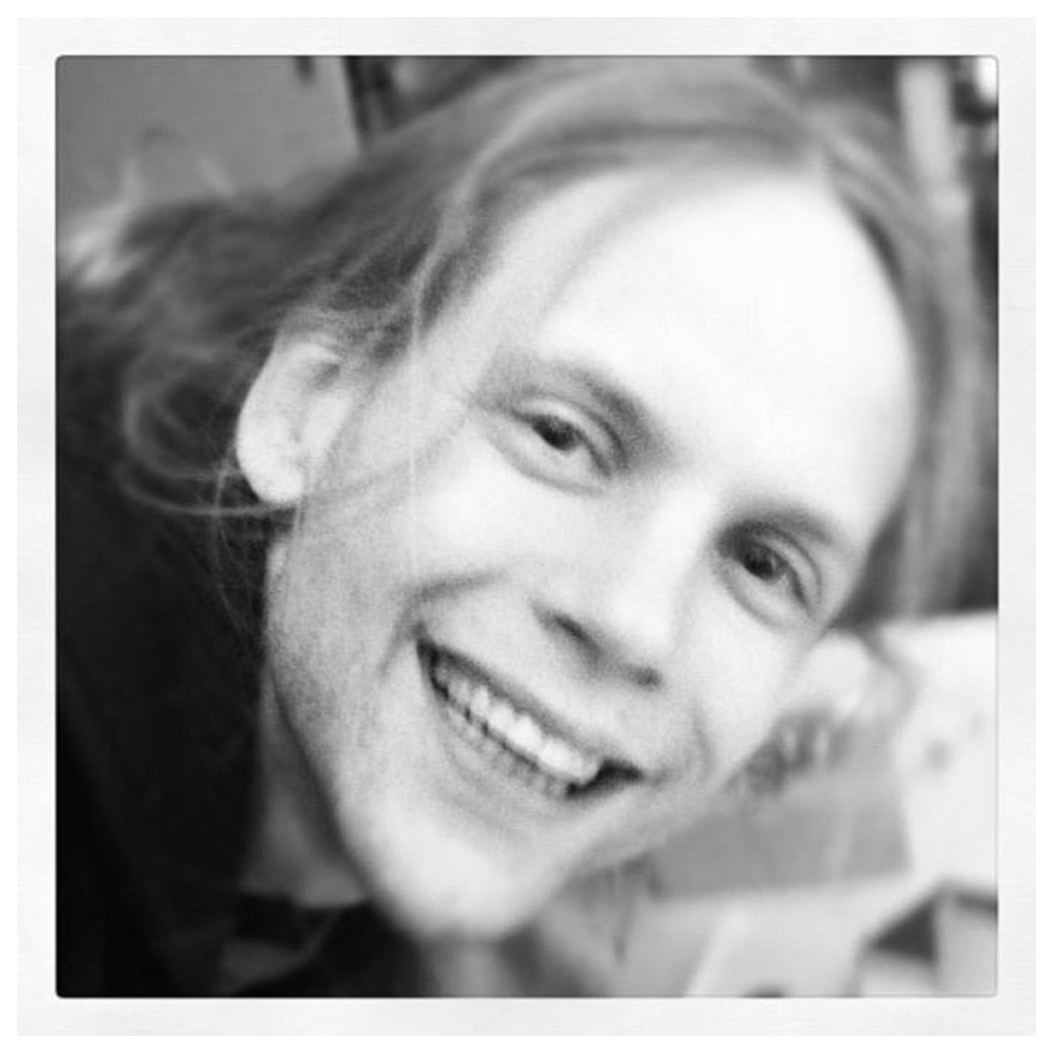
\includegraphics[width=0.3\textwidth]{eps/image_6_1.eps}
\end{wrapfigure}

Danny Arends was born on the 15th of Juli 1983 in the city of Zwolle located in the heart 
of the Netherlands. After moving twice, Danny went to an elementary school situated in 
Heiligerlee, a minuscule hamlet in the north of Holland in the province of Groningen. 

The small school was a perfect match for young Danny during his childhood. Here he quickly 
fell in love with mathematics, and the wondrous world of numbers and patterns. With the 
advent of computers at the elementary school, the love for computers and their inner 
workings also began to develop.

Heiligerlee is located next to a small forest called 'De Hoogte', this forest was used 
by Danny and friends on a daily basis to build tree huts and by using snow balls in winter 
wage war on kids from the other school in Heiligerlee. The forest combined with growing up 
amidst animals on a farm-like residence sparked young Danny his intrests in biology.

After elementary school Danny went to the Ubbo Emmius lyceum in Stadskanaal (Groningen). 
The large scale VWO was a big change compared to the small elementary school. Long hours at school 
together with a long bus ride to and from school, made for long days. Fortunately new 
friends were made in the class room and during the long bus rides. Danny finished high 
school after 6 years, taking mostly exact courses such as mathematics, physics and chemistry.

At 17, a university degree should be the next step in his career. Because of his interests 
in computers, Danny decided that computer science would be a good match. This turned out 
to be not so true. While deeply intrigued by the subject of computational machines, he 
was not satisfied by just studying the workings of a machine build by man.

After two years of Computer science at the University of Groningen, Danny decided it was time 
for a change. Computer science was replaced by Life Science \& Technologie, a bachelor which 
was recently formed as a collaboration between the Biology faculty and Medical Sciences.

He finished his bachelor in record tempo, partly due to the exemptions obtained from 
doing two years of computer science. A Master in molecular biology was quickly selected after
being introduced to bioinformatics at GBIC during a previous bachelor project. The molecular 
biology master allowed for customization of the courses followed, and bioinformatics became the main 
theme in all of the master theses produced. The first thesis: "Machine learning to predict 
transcriptional regulation in prokaryotes" was produced in the group of Oscar Kuipers. 
The second master thesis about 'R/QTL, MQM algorithm' was done in the lab of Ritsert C. Jansen 
under the supervision of Pjotr Prins.

Parts of this second master project are found in this thesis (chapter \ref{chap:mqm}).
After graduating his university master Cum Laude. Danny started a PHD project at Ritsert 
C. Jansen at the Groningen Bioinformatics Centre with a focus on the use of bioinformatic 
tools to handle current challenges in genetics and statistics. These four years of research 
at the GBIC have resulted in the thesis you are currently reading.\\\\

\newpage

\subsection{List of Publications}

\subsubsection*{Authored:}
   R/qtl: high throughput Multiple QTL mapping\\
  \authors{Danny Arends*, Pjotr Prins*, Ritsert C. Jansen and Karl W. Broman}\\
  \bold{Bioinformatics} (2010)\\\\
  Visualizing the genetic landscape of Arabidopsis seed performance\\
  \authors{Ronny V. L. Joosen*, Danny Arends*, Leo Willems, Wilco Ligterink, 
           Henk Hilhorst and Ritsert C. Jansen}\\
  \bold{Plant Physiology} (2011)\\\\
  Large scale NGS pipelines using the MOLGENIS platform: processing the Genome of the Netherlands\\
  \authors{Heorgy V. Byelas*, Danny Arends*, Freerk van Dijk, K. Joeri van der Velde, Laurent 
            Francioli, Martijn Dijkstra, Alexandros Kanterakis, Ishtiaq Ahmad, David van Enckvoort, 
            Leon Mei, Peter Horvatovich, other members of BBMRI-NL, NBIC and Target, Morris A. Swertz}\\
  \bold{Proceeding of: 12th Annual Bioinformatics Open Source Conference BOSC 2011} (2011)\\\\
  xQTL workbench: a scalable web environment for multi-level QTL analysis\\
  \authors{Danny Arends*, K. Joeri van der Velde*, Pjotr Prins, Karl W. Broman, 
           Steffen Moller, Ritsert C. Jansen and Morris A. Swertz}\\
  \bold{Bioinformatics} (2012)\\\\
  WormQTL: Public archive and analysis web portal for natural variation data in Caenorhabditis spp\\
  \authors{L. Basten Snoek*, K. Joeri Van der Velde*, Danny Arends*, Yang Li*, 
           Antje Beyer, Mark Elvin, Jasmin Fisher, Alex Hajnal, Michael O 
           Hengartner, Gino B. Poulin, Miriam Rodriguez, Tobias Schmid, 
           Sabine Schrimpf, Feng Xue, Ritsert C. Jansen, Jan E. Kammenga 
           and Morris A. Swertz}\\
  \bold{Nucleic Acids Research} (2012)\\\\
  Identifying genotype-by-environment interactions in the metabolism of germinating Arabidopsis seeds 
  using Generalized Genetical Genomics\\
  \authors{Ronny V. L. Joosen*, Danny Arends*, Yang Li*, Leo Willems, Joost J. B. Keurentjes, Wilco Ligterink, 
           Ritsert C. Jansen and Henk Hilhorst}\\
  \bold{Plant Physiology} (2013)\\\\
  Cell-type specific eQTL analysis without the need to sort cells\\
  \authors{Harm-Jan Westra*, Danny Arends*, ..., Ritsert C. Jansen and Lude Franke}\\
  \bold{Nature Methods} (2014)

\subsubsection*{Co-Authored:}
  The MOLGENIS toolkit: rapid prototyping of biosoftware at the push of a button\\
  \authors{Morris A Swertz, Martijn Dijkstra, Tomasz Adamusiak,  Joeri K van der Velde, 
           Alexandros Kanterakis, Erik T. Roos, Joris Lops, Gudmundur A. Thorisson, 
           Danny Arends, George Byelas, Juha Muilu, Anthony J. Brookes, Engbert O. de Brock, 
           Ritsert C Jansen and Helen Parkinson}\\
  \bold{BMC Bioinformatics} (2010)\\\\
  XGAP: a uniform and extensible data model and software platform for genotype and phenotype experiments\\
  \authors{Morris A Swertz, K. Joeri van der Velde, Bruno M Tesson, Richard A Scheltema, 
           Danny Arends, Gonzalo Vera, Rudi Alberts, Martijn Dijkstra, Paul Schofield, 
           Klaus Schughart, John M. Hancock, Damian Smedley, Katy Wolstencroft, Carole 
           Goble, Engbert O. de Brock, Andrew R Jones, Helen E Parkinson and Ritsert C Jansen}\\
  \bold{Genome Biology} (2010)\\\\
  SYSGENET: a meeting report from a new European network for systems genetics\\
  \authors{Klaus Schughart, Danny Arends, P. Andreux, R. Balling, Pjotr Prins, et al.}\\
  \bold{Mammalian Genome} (2010)\\\\
  Trans-eQTLs Reveal that Independent Genetic Variants Associated With a Complex Phenotype Converge on 
  Intermediate Genes, with a Major Role for the HLA\\
  \authors{Rudolf SN Fehrmann, Ritsert C. Jansen, Jan H. Veldink, Harm-Jan Westra, Danny Arends,
           Marc Jan Bonder, Jingyuan Fu, Patrick Deelen, Harry J. M. Groen, Asia Smolonska, 
           Rinse K. Weersma, Robert M. W. Hofstra, Wim A. Buurman, ... , Lude Franke}\\
  \bold{Plos Genetics} (2011)\\\\
  Bioinformatics tools and database resources for systems genetics analysis in mice - a short review 
  and an evaluation of future needs\\
  \authors{Caroline Durrant, Morris A. Swertz, Rudi Alberts, Danny Arends, Steffen Möller, 
           Richard Mott, Pjotr Prins, K. Joeri van der Velde, Ritsert C. Jansen and 
           Klaus Schughart}\\
  \bold{Briefings in Bioinformatics} (2011)\\\\
  WormQTLHD - a web database for linking human disease to natural variation data in C. elegans\\
  \authors{K. Joeri van der Velde*, Mark de Haan, Konrad Zych, Danny Arends, L. Basten Snoek, 
           Jan E. Kammenga, Ritsert C. Jansen, Morris A. Swertz and Yang Li}\\
  \bold{Nucleic Acids Research} (2014)

\subsubsection*{In Preparation / Under Review / In Press:}
  Pheno2Geno - High throughput generation of genetic markers and maps from molecular phenotypes\\
  \authors{Konrad Zych, K. Joeri van der Velde, Ronny V. L. Joosen, Wilco Ligterink, Ritsert C Jansen 
           and Danny Arends}\\
  \bold{Submitted}\\\\
  Correlated Traits Locus mapping\\
  \authors{Danny Arends, Pjotr Prins, Harm-Jan Westra, Yang Li, Lude Franke and Ritsert C. Jansen}\\
  \bold{Draft stage}\\\\
  TiQS: web environment for expression QTL analysis\\
  \authors{Steffen M\"oller, Ren\'e Sch\"onfelder, Hajo Krabbenh\"oft, Benedikt Bauer, Yask Gupta, 
           Pjotr Prins, Danny Arends, et al.}\\
  \bold{Submitted}\\\\
  Multiple QTL mapping of cardiac collagen deposition in an F2 population of Scn5a mutant mice reveals 
  interaction between Fgf1 and Pdlim3, Gpr158 \& Itga6\\
  \authors{Elisabeth M. Lodder, Brendon P. Scicluna, L. Beekman, Danny Arends, et al.}\\
  \bold{Submitted}\\\\
  Regulatory Network of Secondary Metabolism in Brassica rapa: An Insight In The Glucosinolate Pathway
  \authors{Dunia Pino del Carpio, Ram Kumar Basnet, Danny Arends, Ke lin, Ric CH de Vos, Dorotha Muth, 
           Jan Kodde, Kim Boutilier, Johan Bucher, Xiaowu Wang, Ritsert Jansen, Guusje Bonnema}\\
  \bold{Submitted}

\subsection*{Acknowledged in:}
  Probability genotype imputation method and integrated weighted lasso for QTL identification\\
  \authors{Nino Demetrashvili, Edwin R van den Heuvel and Ernst C Wit}\\
  \bold{BMC Genetics}, 14:125 (2013)\\\\   
  DesignGG: an R-package and web tool for the optimal design of genetical genomics experiments\\
  \authors{Yang Li, Morris A Swertz, Gonzalo Vera, Jingyuan Fu, Rainer Breitling and Ritsert C Jansen}\\
  \bold{BMC Bioinformatics}, 10:188 (2009)\\\\
  Generalizing genetical genomics: getting added value from environmental perturbation\\
  \authors{Yang Li, Rainer Breitling and Ritsert C. Jansen}\\
  \bold{Trends in Genetics}, 24:518-524 (2008)

\subsection{List of Presentations}
R/xqtl: High throughput modeling, mapping and exploration of Big Data\\
SYSGENET meeting - Braunschweig, April 2010\\\\
Introduction into QTL analysis\\
Dynamic Presentation - University of Groningen, Aug 2010\\\\
MQM and HPC for R/qtl\\
CSBG meeting - Wageningen University, Sept 2010\\\\
Introduction into QTL mapping - Bioinformatics I\\
University of Groningen, June 2011\\\\
(Re)Construction of genetic maps from gene expression data\\
GBIC - University of Groningen, July 2011\\\\
R/qtl for Big Data\\
MIT Department of Biology, invited by Jeroen PJ Saeij\\
MIT, Boston (MA), May 2011\\\\
The Challenge of Big Data Genetical Genomics\\
NCSA, invited by Victor Jongeneel and Chris Fields\\
NCSA, Urbana (IL), May 2011\\\\
Introduction into QTL mapping - Learning From nature (LFN)\\
Wageningen University, Feb 2012\\\\
Computer practical / tutorial - Learning From nature (LFN)\\
Wageningen University, Feb 2012\\\\
Teaching at Summer Course R, R/qtl and GeneNetwork\\
King's college (London, UK), Sept 2013\\\\
Overview R/qtl\\
Humbold University (Berlin, DE), Nov 2013\\\\

\subsection{List of Posters}
User friendly cluster computing for QTL analysis\\
  \authors{Danny Arends, Joeri v/d velde}\\
  \bold{NBIC Conference} April 2010, \& \bold{ISMB} July 2010 - Boston, USA\\\\
Multiple QTL mapping poster\\
  \authors{Danny Arends, Pjotr Prins,Karl W. Broman and Ritsert C. Jansen}\\
  \bold{GBIC day} September 2010 - Groningen, The Netherlands\\\\
Pheno2Geno poster\\
  \authors{Konrad Zych, Danny Arends, Ritsert C. Jansen}\\
  \bold{NBIC} April 2012 - Lunteren, The Netherlands\\\\
Pheno2Geno poster\\
  \authors{Konrad Zych, Danny Arends, Ritsert C. Jansen}\\
  \bold{ECCB / ESCS} Sept 2012 - Basel, Swiss\\\\
GWAS in potato\\
  \authors{Konrad Zych, Danny Arends, Ritsert C. Jansen}\\
  \bold{Kings College} Sept 2013 - London, UK

\subsection{Awards}
1st place Poster Award 'Pheno2Geno' at ESCS2012 Basel (Swiss) (2012)\\
Travel Grant by NBIC for ISMB in Boston (MA, USA) (2010)\\
2nd place Poster Award xQTL workbench NBIC Conference (Lunteren) (2010)\\
Travel Grant 'Short course on system genetics' in Bar Harbor (MA, USA) (2009) by JAX laboratory\\
